\section{UPPER BOUNDS}
\label{sec:upperbounds}

In this section, we present new upper bounds on three variants of PI. We begin by noting that for analysing RPI, Mansour and Singh~\shortcite{Mansour+Singh:1999} deal separately with the cases of $k = 2$ and $k \geq 3$. The main reason for this bifurcation is their use of a specific structural property for $2$-action MDPs. We begin by generalising this property for all $k \geq 2$. Consequently our analysis does not need separate cases, and also yields tighter bounds for $k \geq 3$.

%\begin{definition}
%    For a policy $\pi$ and state $s$, we define the set of improvable actions at $s$ as $T^{\pi}(s) = \{a | Q^{\pi}(s,a)>V^{\pi}(s) \vee (Q^{\pi}(s,a)=V^{\pi}(s) \wedge a\ge\pi(s)) \}$.
%\end{definition}

%In particular, note that $\pi(s) \in T^\pi(s)$.

\begin{lemma}
\label{lem:bijection}
    For policies $\pi_1, \pi_2 \in \Pi$, if $|T^{\pi_1}(s)|=|T^{\pi_2}(s)|$ for all states $s \in S$, then $\pi_1=\pi_2$.
\end{lemma}

\begin{proof}
    Assume that $|T^{\pi_1}(s)|=|T^{\pi_2}(s)|$ for some policies $\pi_1$ and $\pi_2$, for all states $s$. Now, for each state $s$, note that $A \setminus T^{\pi_{1}}(s)$ and $T^{\pi_{2}}(s) \cup \{\pi_{2}(s)\}$ cannot be disjoint, since that would imply $(T^{\pi_{2}}(s) \cup \{\pi_{2}(s)\}) \subseteq T^{\pi_{1}}(s)$, which cannot be true since $|T^{\pi_{2}}(s) \cup \{\pi_{2}(s)\}| = 1 +  |T^{\pi_{1}}(s)|$. Hence, we may construct a policy $\pi_{3}$ such that for each state $s$, $\pi_{3}(s) \in  (A \setminus T^{\pi_{1}}(s))\cap (T^{\pi_{2}}(s) \cup \{\pi_{2}(s)\})$. By Theorem~\ref{thm:pi}, it follows that $\pi_3 \gtrsim \pi_2$. Similarly, by Corollary~\ref{cor:pd}, it must be that $\pi_{1} \gtrsim \pi_{3}$. Hence, $\pi_{1} \gtrsim \pi_{3} \gtrsim \pi_{2}$. Now, if we construct a policy $\pi_{4}$ such that for each state $s$, $\pi_{4}(s) \in  (A \setminus T^{\pi_{2}}(s))\cap (T^{\pi_{1}}(s) \cup \{\pi_{1}(s)\})$, a similar argument yields $\pi_{2} \gtrsim \pi_{4} \gtrsim \pi_{1}$. Since $\pi_{2} \gtrsim \pi_{1}$ and $\pi_{1} \gtrsim \pi_{2}$, we get $\pi_{1} = \pi_{2}$.
    %and by policy deprovement theorem, $\pi_1 \succeq \pi_3$. Therefore $\pi_1 \succeq \pi_2$. Similarly, we can construct $\pi_4$ such that $\pi_2 \succeq \pi_4 \succeq \pi_1$. So we have $\pi_1 \preceq \pi_2$ and $\pi_1 \succeq \pi_2$, implying $V^{\pi_1} \preceq V^{\pi_2}$ and $V^{\pi_1} \succeq V^{\pi_2}$. Thus $V^{\pi_1}=V^{\pi_2}$ and hence $Q^{\pi_1}=Q^{\pi_2}$. This implies $\pi_1=\pi_2$. For the sake of contradiction, assume $\pi_1(s)>\pi_2(s)$ for some state $s$. Then $a\in T^{\pi_1}(s) \Rightarrow Q^{\pi_1}(s,a)>V^{\pi_1}(s) \vee (Q^{\pi_1}(s,a)=V^{\pi_1}(s) \wedge a\ge\pi_1(s)) \Rightarrow Q^{\pi_2}(s,a)>V^{\pi_2}(s) \vee (Q^{\pi_2}(s,a)=V^{\pi_2}(s) \wedge a\ge\pi_2(s)) \Rightarrow a \in T^{\pi_2}(s)$. Also $\pi_2(s)\in T^{\pi_2}(s)$ but $\pi_2(s)\notin T^{\pi_1}(s)$. Thus $T^{\pi_1}(s)\subsetneq T^{\pi_2}(s)$ contradicting $|T^{\pi_1}(s)|=|T^{\pi_2}(s)|$.
    % Now, if $\pi_1(s)\ne \pi_2(s)$ for some state $s$, it is easy to show that $|T^{\pi_1}(s)|\ne |T^{\pi_2}(s)|$. Hence we must have $\pi_1=\pi_2$. 
\end{proof}


The lemma establishes that for a given policy $\pi \in \Pi$, the sequence $(|T^{\pi}(s)|)_{s \in S}$ is unique. Since $0 \leq |T^{\pi}(s)| \leq k - 1$, the number of possible sequences is $k^{n}$. As the number of policies is also $k^{n}$, we have a bijection between $\Pi$ and this set of ``improvement sequences''. This connection was already known for $k = 2$~\cite{Mansour+Singh:1999,Szabo+Welzl:2001}, which is simpler to analyse because $|T^{\pi}(s)| \in \{0, 1\}$ becomes an indicator for whether $s$ is improvable. Our generalisation for all $k \geq 2$ is novel. Our use of $\gtrsim$, which break ties, gives Lemma~\ref{lem:bijection} the convenient form of a bijection. Our analysis can also be undertaken using only $\succ$ and $\succeq$, albeit with extra cases to account for ties.

\subsection{Improving over RPI's Upper Bound}

%It follows from Theorem X that for a given policy $\pi$, there is a set of policies $I(\pi)$, with $|I(\pi)| = \prod_{s \in S}|T^{\pi}(s) + 1| - 1$, such that for each $\pi^{\prime} \in I(\pi)$, $\pi^{\prime} \gtrsim \pi$, and $\pi^{\prime} = \textsf{modify}(\pi, U)$ for a suitable choice of $U$. 


In order to effectively use Lemma~\ref{lem:bijection}, we propose a slight modification to RPI. In the new variant, denoted RPI-UIP, $\pi^{\prime}$ is picked uniformly at random from $I(\pi)$, the set of improving policies. Even if $I(\pi)$ itself is exponentially large, note that it ``factors'' into improvements at each state, and so 
only a polynomial-time operation is needed to pick $\pi^{\prime}$ uniformly at random from $I(\pi)$.


RPI-UIP is identical to RPI on $2$-action MDPs, but since RPI picks uniformly at random among the improvable \textit{states} (and picks improving actions arbitrarily), the methods do not coincide for $k \geq 3$. 
Lemma~\ref{lem:bijection} facilitates a tighter bound for RPI-UIP when used in conjunction with the analysis structure of Mansour and Singh~\shortcite{Mansour+Singh:1999}.

\begin{definition}
A policy $\pi$ is called a small-improvement policy if $|I(\pi)| \leq \alpha$ (we shall fix the parameter $\alpha > 0$ subsequently). A policy that is not a small-improvement policy is called a large-improvement policy.
\end{definition}


%Here, $t \in \mathbb{R}_{>0}$ is a parameter which we will fix later.
We present a novel bound on the number of small-improvement policies. This bound is slightly looser than the specialised one derived by Mansour and Singh~\shortcite{Mansour+Singh:1999} for $k = 2$, but is tighter than theirs for $k \geq 3$.

\begin{lemma}
\label{lem:countsmall}
    For all $\alpha > 0$, there are at most $(\alpha + 1)H_{k}^{n-1}$ small-improvement policies, where $H_k = \sum_{i=1}^{k} \frac{1}{i}$. Note that $H_{k} = \Theta(\log k)$.
\end{lemma}
\begin{proof}
    For convenience we take $S = \{1, 2, \dots, n\}$. The bijection in  Lemma~\ref{lem:bijection} allows us to associate each policy $\pi$ with a unique $n$-length, $k$-ary string $x^{\pi}$ of the form $x^{\pi}_{1}x^{\pi}_{2}\dots{x^{\pi}_{n}}$, wherein for s $\in S$, $x^{\pi}_{s} = |T^{\pi}(s)| + 1$. It is immediate that $|I(\pi)| = \prod_{i = 1}^{n} x^{\pi}_{i} - 1$. Thus, $\pi$ is a small-improvement policy if and only if
    $\prod_{i = 1}^{n} x^{\pi}_{i} \leq \alpha + 1.$ For $\beta > 0$, let $N(n, \beta)$ denote the number of $n$-length strings over \{1, 2, \dots, k\}---of the form $x = x_{1}x_{2}\dots{x_{n}}$---for which $\prod_{i = 1}^{n} x_{i} \leq \beta.$ To prove the lemma, we induct on $n$ to show that $N(n, \beta) \leq \beta H_{k}^{n - 1}$.
  
    Clearly for all $\beta > 0$, $N(1, \beta) = \min(\lfloor\beta\rfloor, k) \leq \beta$.
    %Formally, $f(n,t) = |\{\pi \in \Pi: \prod_{s\in S}|T^\pi(s)| \le t\}| = |\{v\in [k]^n : \prod_{i=1}^{n}v_i \le t\}|$. 
    %We induct on the number of states in the MDP. For a single-state MDP, the improvement-sequences are $0, 1, \dots, k - 1$, and so $X(1, \alpha) = \min(\floor{\alpha}, k - 1) \leq \alpha$ for all $\alpha > 0$. %
Now assume that for all $\beta > 0$ and some $n \geq 1$, $N(n, \beta) \leq \beta H_k^{n - 1}$. For $l \in \{1, 2, \dots, k\}$, consider $N(n + 1, \beta, x_{1} = l)$, the number of $(n + 1)$-length strings in which the first element is $l$ and $\prod_{i = 1}^{n + 1} x_{i} \leq \beta.$ We have: (1) 
$N(n + 1,\beta) = \sum_{l = 1}^{k} N(n + 1, \beta, x_{1} = l)$, and (2) $N(n + 1, \beta, x_{1} = l) = N(n, \frac{\beta}{l})$. Applying the induction hypothesis, we get $N(n + 1,\beta) \leq \sum_{l = 1}^{k} \frac{\beta}{l} H_{k}^{n - 1} = \beta H_{k}^{n}$, which completes the proof.
\end{proof}
Next we lower-bound the progress made by each step of RPI-UIP. By  constructing a total order, we obtain a simpler proof of the following lemma than the one given by
Mansour and Singh~\shortcite[see Lemma 9]{Mansour+Singh:1999}.
\begin{lemma}
\label{lem:largeimp}
%If $\pi$ is a large improvement policies, and $\pi'$ is obtained from $\pi$ by applying randomized policy iteration, the expected number of policies $\pi''$ such that $\pi \preceq \pi'' \prec \pi'$ is more than $\frac{t}{2}$.
Let $\pi^{\prime}$ be the policy obtained by performing policy improvement to a policy $\pi$ using RPI-UIP. Then, with probability at least $\frac{1}{2}$, there exist $\lfloor \frac{|I(\pi)|}{2} \rfloor$ policies $\pi^{\prime\prime} \neq \pi$ such that $\pi^{\prime\prime} \gtrsim \pi$ and $\neg(\pi^{\prime\prime} \gtrsim \pi^{\prime})$.
\end{lemma}
\begin{proof}
%The number of available choices for $\pi'$ is more than $t$ for a large improvement policy. If one is selected from these uniformly at random, the expected number of policies $\pi''$ such that $\pi'' \preceq \pi$ and $\pi''$ improves upon $\pi$ is half of the total number.
We define a relation $R$ between policies: $\pi_{1}R\pi_{2} \iff (\pi_{1} \gtrsim \pi_{2}) \vee (\neg(\pi_{1} \gtrsim \pi_{2}) \wedge (\pi_{1}L\pi_{2}))$. Observe that $R$ induces a total order on $\Pi$, and therefore on $I(\pi)$. Since $\pi^{\prime}$ is picked uniformly at random from $I(\pi)$, with probability at least $1/2$, we will have $\pi^{\prime}R \pi^{\prime\prime}$---which implies $\neg(\pi^{\prime\prime} \gtrsim \pi^{\prime})$---for some  $\lfloor |I(\pi)| / 2 \rfloor$ policies $\pi^{\prime\prime}$. Since 
$\pi^{\prime\prime} \in I(\pi)$, we have
$\pi^{\prime\prime} \neq \pi$, and by Theorem~\ref{thm:pi}, $\pi^{\prime\prime} \gtrsim \pi.$
\end{proof}
We are ready to upper-bound the complexity of RPI-UIP.
\begin{theorem}
The expected number of policies evaluated by RPI-UIP is at most $O(k^{n/2}H_{k}^{(n - 1)/2})$.
\end{theorem}
\begin{proof}
Define $L^{\star} = k^{n}/\lfloor \alpha / 2\rfloor$. Since each large-improvement policy eliminates at least
$\lfloor \alpha / 2\rfloor$ policies with probability at least $1/2$, and in total there are $k^{n}$ policies, the expected number of large-improvement policies visited is at most $2L^{\star}$. 
%Hence, the expected number of large-improvement policies evaluated is at most $6L^{\star} + 0.51^{L^{\star}}k^{n}$.
By Lemma~\ref{lem:countsmall},
the total number of small-improvement policies is at most $(\alpha + 1)H_{k}^{n - 1}$.
Taking $\alpha = \sqrt{k^{n} / H_k^{n-1}}$, we obtain a bound of $O(k^{n/2}H_{k}^{(n - 1)/2})$ on the expected iterations of RPI-UIP. Note that the number of iterations decays exponentially:
the probability that $6L^{\star}$ large-improvement policies are visited is upper-bounded by  ${6L^{\star} \choose 5L^{\star}}\left(\frac{1}{2}\right)^{5L^{\star}} = {6L^{\star} \choose L^{\star}}\left(\frac{1}{2}\right)^{5L^{\star}} \leq \left(\frac{6e}{32}\right)^{L^{\star}} < 0.51^{L^{\star}}$.%\qedhere
%Substituting $H_{k} = O(\log(k))$ completes the proof.
\end{proof}
Whereas RPI is shown to eliminate $(\Theta(1))^{n}$ policies in large-improvement steps~\cite{Mansour+Singh:1999}, we have shown that RPI-UIP eliminates $(\text{poly}(k))^{n}$ policies in such steps---which leads to the tighter upper bound.
%Note that since $I(\pi)$ is ``factored'' into improvements at each state, only a polynomial operation is needed to pick $\pi^{\prime}$ uniformly at random from $I(\pi)$, even if $I(\pi)$ itself is exponentially large.


\begin{comment}

% We say that an improvement is large if it rules out at least $\frac{1}{4}(\kappa k) ^ {\eta n}$ policies. This happens with probability
\begin{theorem}
    With probability $1-e^{-\Omega(k^{0.5n})}$, randomized policy iteration visits at most $8 k^{\frac{n}{2}}H_k^\frac{n-1}{2}$ iterations.
\end{theorem}

\begin{proof}
With probability at least $\frac{1}{3}$
we rule out more than $\frac{t}{4}$ policies, at a large improvement policy. (If this occurs
with probability strictly less than $\frac{1}{3}$, then the expected
number of policies we rule out is less than or equal to
$\frac{1}{3}\cdot t + \frac{2}{3}\cdot\frac{t}{4} = \frac{t}{2}$, which contradicts
the Lemma \ref{lem:largeimp}.) 

An improvement of a policy is good if it rules out more than $\frac{t}{4}$ policies. The probability that a large improvement policy gets a good improvement is at least
$\frac{1}{3}$. A run that visits $L$ large improvement policies is called typical if at least $\frac{L}{4}$ of these
$L$ policies cause good improvements. The number
of good improvements in a run is bounded by
$\frac{4 k^n}{t}$. Hence a typical run can visit at most $4\cdot\frac{4 k^n}{t}=\frac{16 k^n}{t}$ large improvement policies. Total number of policies visited by a typical run is bounded by
$t H_k^{n-1}+\frac{16 k^n}{t}$. Setting $t=4\sqrt{\frac{k^n}{H_k^{n-1}}}$ gives us the bound
$N = 8 k^{\frac{n}{2}}H_k^\frac{n-1}{2}$.

If a run visits more than $N$ policies, it can not be typical.
The probability that a run is not typical and visits $L>N$ policies is at most $e^{-2(\frac{1}{3}-\frac{1}{4})^2 L} = e^{-\frac{L}{72}} < e^{-\frac{N}{72}}=e^{-\Omega(k^{0.5n})}$.

\end{proof}


\end{comment}

\subsection{A new upper bound for HPI}

In HPI, every improvable state must necessarily be switched. Yet, for $k \geq 3$, there could sometimes be two or more improving actions for a particular state---so there is still a choice to resolve. We propose HPI-R, a variant of HPI, in which an improving action is picked uniformly at random from those available for every improvable state. Equivalently, let us say that a policy $\pi^{\prime}$ \textit{strictly improves} upon a policy $\pi$ if $\forall s\in S: (\pi^{\prime}(s) \in (T^\pi(s) \cup \{\pi(s)\})) \wedge (\pi^{\prime}(s)=\pi(s)\Rightarrow |T^\pi(s)|=0)$. Let $I_{\text{strict}}(\pi)$ be the set of all policies that strictly improve upon $\pi$. HPI-R picks an improving policy $\pi^{\prime}$ uniformly at random from $I_{\text{strict}}(\pi)$. The crux of our analysis is that $I_{\text{strict}}(\pi)$ is still sufficiently large if $I(\pi)$ is large. If $\pi$ is optimal, $I_{\text{strict}}(\pi) = I(\pi) = \emptyset$, else
\begin{align*}
|I_{\text{strict}}(\pi)|
&= \prod_{s \in S} \max(|T^{\pi}(s)|, 1)
\geq
\prod_{s \in S} \left(\frac{|T^{\pi}(s)| + 1}{2}\right)\\
&\geq
\frac{\prod_{s \in S} (|T^{\pi}(s)| + 1) - 1}{2^{n}}
=  \frac{|I(\pi)|}{2^{n}}.
\end{align*}
With this connection established, we can use the same analysis structure as before. With probability at least $1/2$, HPI-R eliminates  $\lfloor I(\pi) / 2^{n + 1} \rfloor$ policies after visiting $\pi$. Taking $\alpha = \sqrt{2^{n}k^{n}/H_{k}^{n - 1}}$, we obtain the following upper bound.
\begin{theorem}
The expected number of policies evaluated by HPI-R is at most $O(2^{n/2}k^{n/2}H_{k}^{(n - 1)/2})$.
\end{theorem}
For $k \geq 5$, this bound marks an exponential improvement over the previous bound of $O(k^{n}/n)$ for HPI~\cite{Mansour+Singh:1999}. 

% \begin{comment}
% \begin{lemma}
% \label{lem:largesimp}
%     If $\pi$ is a large improvement policies, and $\pi'$ is obtained from $\pi$ by applying Howard's policy iteration, the expected number of policies $\pi''$ such that $\pi \preceq \pi'' \prec \pi'$ is more than $\frac{t}{2^{n+1}}$.
% \end{lemma}

% \begin{proof}
%     The number of available choices for $\pi'$ is more than $\frac{t}{2^{n}}$ for a large improvement policy. If one is selected from these uniformly at random, the expected number of policies $\pi''$ such that $\pi'' \preceq \pi$ and $\pi''$ improves upon $\pi$ is half of the total number.
% \end{proof}

% \begin{theorem}
%     With probability $1-e^{-\Omega(k^{0.5n})}$, randomized Howard's policy iteration visits at most $8 \cdot 2^{\frac{n}{2}}k^{\frac{n}{2}}H_k^\frac{n-1}{2}$ iterations.
% \end{theorem}

% \begin{proof}
% With probability at least $\frac{1}{3}$
% we rule out more than $\frac{t}{2^{n+2}}$ policies, at a large improvement policy. (If this occurs
% with probability strictly less than $\frac{1}{3}$, then the expected
% number of policies we rule out is less than or equal to
% $\frac{1}{3}\cdot \frac{t}{2^{n}} + \frac{2}{3}\cdot\frac{t}{2^{n+2}} = \frac{t}{2^{n+1}}$, which contradicts
% the Lemma \ref{lem:largesimp}.) 

% An improvement of a policy is good if it rules out more than $\frac{t}{2^{n+2}}$ policies. The probability that a large improvement policy gets a good improvement is at least
% $\frac{1}{3}$. A run that visits $L$ large improvement policies is called typical if at least $\frac{L}{4}$ of these
% $L$ policies cause good improvements. The number
% of good improvements in a run is bounded by
% $4\cdot \frac{2^n k^n}{t}$. Hence a typical run can visit at most $4\cdot 4\cdot \frac{2^n k^n}{t}=16\cdot\frac{2^n k^n}{t}$ large improvement policies. Total number of policies visited by a typical run is bounded by
% $t H_k^{n-1}+16\cdot\frac{2^n k^n}{t}$. Setting $t=4\sqrt{\frac{2^n k^n}{H_k^{n-1}}}$ gives us the bound
% $N = 8\cdot 2^{\frac{n}{2}} k^{\frac{n}{2}}H_k^\frac{n-1}{2}$.

% If a run visits more than $N$ policies, it can not be typical.
% The probability that a run is not typical and visits $L>N$ policies is at most $e^{-2(\frac{1}{3}-\frac{1}{4})^2 L} = e^{-\frac{L}{72}} < e^{-\frac{N}{72}}=e^{-\Omega(k^{0.5n})}$.
% \end{proof}

% \end{comment}


\subsection{Tighter bounds for BSPI}

The tightest strong bound yet for deterministic PI variants is achieved by
BSPI~\cite{Kalyanakrishnan+MG-bspi:2016}. Assume $S$ is partitioned arbitrarily into $\lceil n/b \rceil$ $b$-sized batches (with one batch possibly smaller). If the batches are indexed, then at each iteration, 
BSPI selects the highest-indexed batch $B \subseteq S$ that has improvable states, and switches \textit{all} the improvable states in $B$. This operation can be viewed as performing HPI within $B$. The analysis of BSPI rests on a recursive argument that if $\tau(b)$ is an upper bound on the iterations taken by HPI on a $b$-state MDP, then BSPI with a batch size of $b$ on an $n$-state MDP will take at most $\tau(b)^{\lceil n/b \rceil}$ iterations. While the original analysis was for $2$-action MDPs~\cite{Kalyanakrishnan+MG-bspi:2016}, a carefully-designed recursion over actions is shown to yield an upper bound of $k^{\lceil n/b \rceil \log_{2}\tau(b)}$ iterations for $k$-action MDPs~\cite{Kalyanakrishnan+Gupta}. Using the order regularity relaxation to bound $\tau(b)$, a computer search shows $\tau(7) \leq 33$~\cite{Gerencser+HDJ:2015}.

We obtain tighter bounds for BSPI by enumerating all possible AUSOs of dimension up to 4 (the number of AUSOs is doubly-exponential in the dimension, and currently infeasible to enumerate for dimension $5$). We directly calculate the number of evaluations performed by HPI starting at each possible vertex on each AUSO; this number is guaranteed not to exceed the order regularity bound. Interestingly, we can also test which AUSOs satisfy the Holt-Klee conditions, possibly further tightening the upper bound applicable to MDPs.

Ignoring isomorphisms, there are $18$ AUSOs in dimension $3$ (or ``$3$-AUSOs''), of which $16$ satisfy the Holt-Klee conditions.\footnote{Of the $19$ oriented $3$-cubes listed by Stickney and Watson~\shortcite[see Figure 3]{Stickney+Watson:1978}, the $19^{\text{th}}$ contains a cycle.} There are instances of both types of AUSOs on which HPI can perform $5$ evaluations, matching the bound from the order regularity problem. A more interesting fact emerges from the set of $4$-AUSOs. There are 12640 $4$-AUSOs, of which $6113$ satisfy the Holt-Klee conditions. For the latter set, HPI never needs more than $7$ evaluations. Hence, we obtain $7^{n/4} < 1.6266^{n}$ iterations as a bound for BSPI with $b = 4$ on $2$-action MDPs, which improves upon the existing bound of $33^{n/7} < 1.6479^{n}$. The corresponding improvement for $k$-action MDPs is a bound of $k^{0.7019n}$ iterations in place of $k^{0.7207n}$~\cite{Kalyanakrishnan+Gupta}. HPI never performs more than $8$ evaluations on $4$-AUSOs; indeed there is only one $4$-AUSO on which it performs $8$ evaluations. This AUSO, shown in Appendix~\ref{app:upperbounds} (see supplementary material), does not satisfy the Holt-Klee conditions.


% % Moved to appendix


 \begin{figure}[H]
 \centering
\scalebox{0.7}
% \scalebox{0.5}
 {
 \begin{tikzpicture}[scale=2.5]
    

\pgfarrowsdeclare{mytipnew}{mytipnew} 
{ 
  \arrowsize=0.2pt 
  \advance\arrowsize by .5\pgflinewidth 
  \pgfarrowsleftextend{-4\arrowsize-2\pgflinewidth} 
  \pgfarrowsrightextend{2\pgflinewidth} 
} 
{ 
  \arrowsize=1pt 
  \advance\arrowsize by .5\pgflinewidth 
  \pgfsetdash{}{0pt} % do not dash 
  \pgfsetroundjoin   % fix join 
  \pgfsetroundcap    % fix cap 
  \pgfpathmoveto{\pgfpoint{-4\arrowsize}{3\arrowsize}}
  \pgfpathlineto{\pgfpoint{4\arrowsize}{0\arrowsize}}
  \pgfpathlineto{\pgfpoint{-4\arrowsize}{-3\arrowsize}}
  \pgfpathlineto{\pgfpoint{0\arrowsize}{0\arrowsize}}
  \pgfpathlineto{\pgfpoint{-4\arrowsize}{3\arrowsize}}
%   \pgfusepathqstroke 
  \pgfusepathqfill
}
 \tikzset{
  % style to apply some styles to each segment of a path
  every node/.style={draw,circle,inner sep=0pt,minimum size=0pt},
  on each segment/.style={
     decorate,
     decoration={
      show path construction,
      moveto code={},
      lineto code={
         \path [#1]
         (\tikzinputsegmentfirst) -- (\tikzinputsegmentlast);
      },
      curveto code={
         \path [#1] (\tikzinputsegmentfirst)
         .. controls
         (\tikzinputsegmentsupporta) and (\tikzinputsegmentsupportb)
         ..
         (\tikzinputsegmentlast);
      },
      closepath code={
         \path [#1]
         (\tikzinputsegmentfirst) -- (\tikzinputsegmentlast);
      },
     },
  },
  mid arrow/.style={postaction={decorate,decoration={
         markings,
         mark=at position .5 with {{\arrow[#1]{mytipnew}}},
      }}},
  near arrow/.style={postaction={decorate,decoration={
         markings,
         mark=at position .4 with {{\arrow[#1]{mytipnew}}},
      }}},
  far arrow/.style={postaction={decorate,decoration={
         markings,
         mark=at position .6 with {{\arrow[#1]{mytipnew}}},
      }}},
 }


\tikzstyle{edge} = [draw,thick,postaction={on each segment={mid arrow=black}},black]
\tikzstyle{edgefar} = [draw,thick,postaction={on each segment={far arrow=black}},black]
\tikzstyle{edgenear} = [draw,thick,postaction={on each segment={near arrow=black}},black]
\newcommand{\mycircle}[1]{\large{\raisebox{.5pt}{\textcircled{\raisebox{-.9pt} {#1}}}}}
\path(0,0) node[label=below right:{\mycircle{8}}] (v0) {}
     (0,1) node (v1)[label=below left:\mycircle{7}] {}
     (1,0) node (v2) {}
     (1,1) node (v3) {}
     (0.23, 0.4) node (v4)[label=below right:\mycircle{1}] {}
     (0.23,1.4) node (v5) {}
     (1.23,0.4) node (v6) {}
     (1.23,1.4) node (v7)[label=above left:\mycircle{3}] {}
     (-1,-1) node (v8) {}
     (-1,2) node (v9)[label=above left:\mycircle{6}] {}
     (-0.66,2.7) node (v13)[label=above left:\mycircle{5}] {}
     (-0.66,-0.3) node (v12) {}
     (2,-1) node (v10)[label=below right:\mycircle{2}] {}
     (2.34,-0.3) node (v14) {}
     (2,2) node (v11)[label=below right:\mycircle{4}] {}
     (2.34,2.7) node (v15) {};
% \node[above of=v1,node distance=0.2in] (v1l) {2};
\draw[edge]
%  (v1) -- (v0)
 (v2) -- (v0)
%  (v2) -- (v3)
 (v3) -- (v1)
 (v3) -- (v11)
 (v4) -- (v0)
 (v4) -- (v6)
 (v4) -- (v12)
 (v5) -- (v1)
%  (v5) -- (v4)
 (v5) -- (v7)
%  (v5) -- (v13)
 (v6) -- (v2)
%  (v6) -- (v7)
 (v7) -- (v3)
%  (v7) -- (v15)
 (v8) -- (v0)
 (v8) -- (v9)
 (v8) -- (v10)
 (v9) -- (v1)
 (v10) -- (v2)
 (v10) -- (v11)
 (v10) -- (v14)
 (v11) -- (v9)
 (v11) -- (v15)
 (v12) -- (v8)
 (v12) -- (v13)
 (v12) -- (v14)
 (v13) -- (v9)
 (v14) -- (v6)
 (v14) -- (v15)
 (v15) -- (v13);
 \draw[edgenear] (v5) -- (v13) (v7) -- (v15) (v1) -- (v0) (v6) -- (v7);
 \draw[edgefar] (v2) -- (v3) (v5) -- (v4);
    %  \draw[edge] (v1) -- (v0);
    %  \draw[edge] (v2) -- (v0);
    %  \draw[edge] (v2) -- (v3);
    %  \draw[edge] (v3) -- (v1);
    %  \draw[edge] (v3) -- (v11);
    %  \draw[edge] (v4) -- (v0);
    %  \draw[edge] (v4) -- (v6);
    %  \draw[edge] (v4) -- (v12);
    %  \draw[edge] (v5) -- (v1);
    %  \draw[edge] (v5) -- (v4);
    %  \draw[edge] (v5) -- (v7);
    %  \draw[edge] (v5) -- (v13);
    %  \draw[edge] (v6) -- (v2);
    %  \draw[edge] (v6) -- (v7);
    %  \draw[edge] (v7) -- (v3);
    %  \draw[edge] (v7) -- (v15);
    %  \draw[edge] (v8) -- (v0);
    %  \draw[edge] (v8) -- (v9);
    %  \draw[edge] (v8) -- (v10);
    %  \draw[edge] (v9) -- (v1);
    %  \draw[edge] (v10) -- (v2);
    %  \draw[edge] (v10) -- (v11);
    %  \draw[edge] (v10) -- (v14);
    %  \draw[edge] (v11) -- (v9);
    %  \draw[edge] (v11) -- (v15);
    %  \draw[edge] (v12) -- (v8);
    %  \draw[edge] (v12) -- (v13);
    %  \draw[edge] (v12) -- (v14);
    %  \draw[edge] (v13) -- (v9);
    %  \draw[edge] (v14) -- (v6);
    %  \draw[edge] (v14) -- (v15);
    %  \draw[edge] (v15) -- (v13);
    %  \draw[selected edge] (v4) -- (v10);
    %  \draw[selected edge] (v10) -- (v7);
    %  \draw[selected edge] (v7) -- (v11);
    %  \draw[selected edge] (v11) -- (v13);
    %  \draw[selected edge] (v13) -- (v9);
    %  \draw[selected edge] (v9) -- (v1);
    %  \draw[selected edge] (v1) -- (v0);
 \end{tikzpicture}
 }
 \caption{The only 4-AUSO (up to an isomorphism) on which HPI performs $8$ vertex evaluations. The $8$ vertices are numbered in sequence. This AUSO does not satisfy the Holt-Klee conditions. Notice, for example, that the inner $3$-AUSO does not have $3$ vertex-disjoint paths from source to sink.}
 \label{fig:4auso-8hpi}
\end{figure}


While the improved upper bounds above become the tightest strong worst-case bounds known for the PI family (since HPI is deterministic), our enumerated list of AUSOs also facilitates the analysis of a randomised variant of BSPI in which RPI is used within each batch. We denote this variant BSPI-R. We are not aware of relaxations such as the order regularity problem for analysing BSPI-R; our direct enumeration of AUSOs provides the first non-trivial bounds. We find that the expected number of iterations RPI takes on $3$-AUSOs is at most $4.7778$ and on $4$-AUSOs is at most $6.5544$ (in both cases the Holt-Klee conditions do not lead to tighter bounds). Although these bounds---maximised over all AUSOs in the corresponding family---are smaller than those for HPI, there do exist AUSOs on which HPI dominates RPI. The distributions of the number of iterations taken by RPI and HPI on $3$- and $4$-AUSOs are shown in Figure~\ref{fig:3-4-auso-bounds}. Reusing the recursion shown by Kalyanakrishnan \textit{et al.}~\shortcite{Kalyanakrishnan+MG-bspi:2016}, we obtain $6.5544^{n/4} < 1.6001^{n}$ as a bound on the number of iterations taken by BSPI-R on $2$-action MDPs. This strong upper bound is the tightest shown to date for the PI family for $k = 2$. 
%The generalisation---$k^{0.6782n}$ for $k$-action MDPs---is not as tight as 
For $k \geq 3$, %the $(O(\log k))^{n}$ bound of Gupta and Kalyanakrishnan~\shortcite{Kalyanakrishnan+Gupta} is 
the tightest such bounds are
$(O(\log k))^{n}$~\cite{Kalyanakrishnan+Gupta}.


\begin{figure}[t]
\centering%%% not \center
\mbox{
\subfigure[3-AUSO]{%
\label{fig:auso3}%
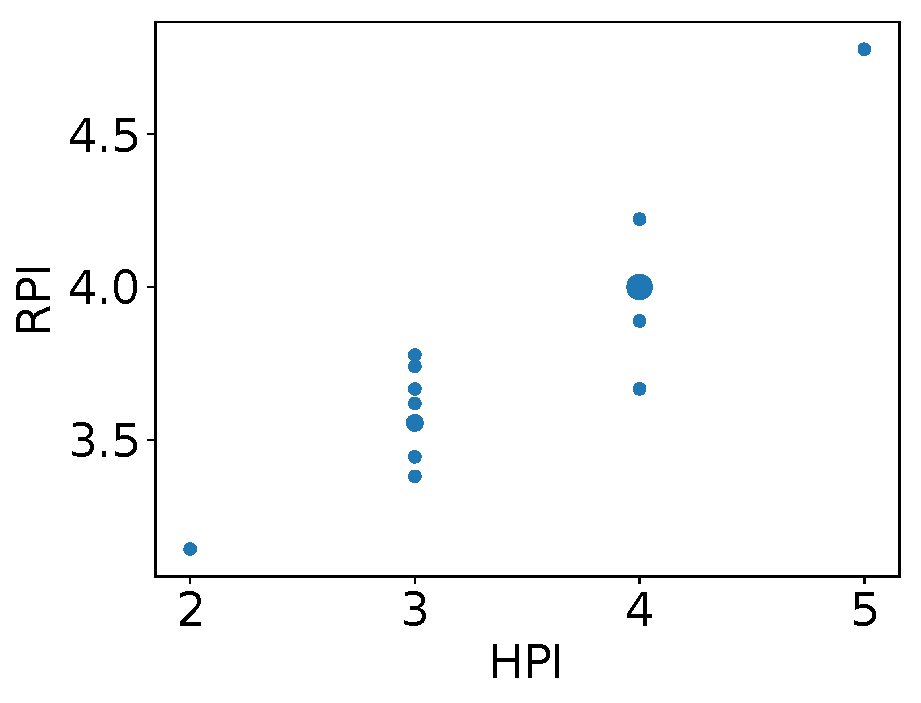
\includegraphics[width=0.24\textwidth]{figs/3-auso-scatter}%
}%
\subfigure[3-AUSO (Holt-Klee)]{%
\label{fig:hkauso3}%
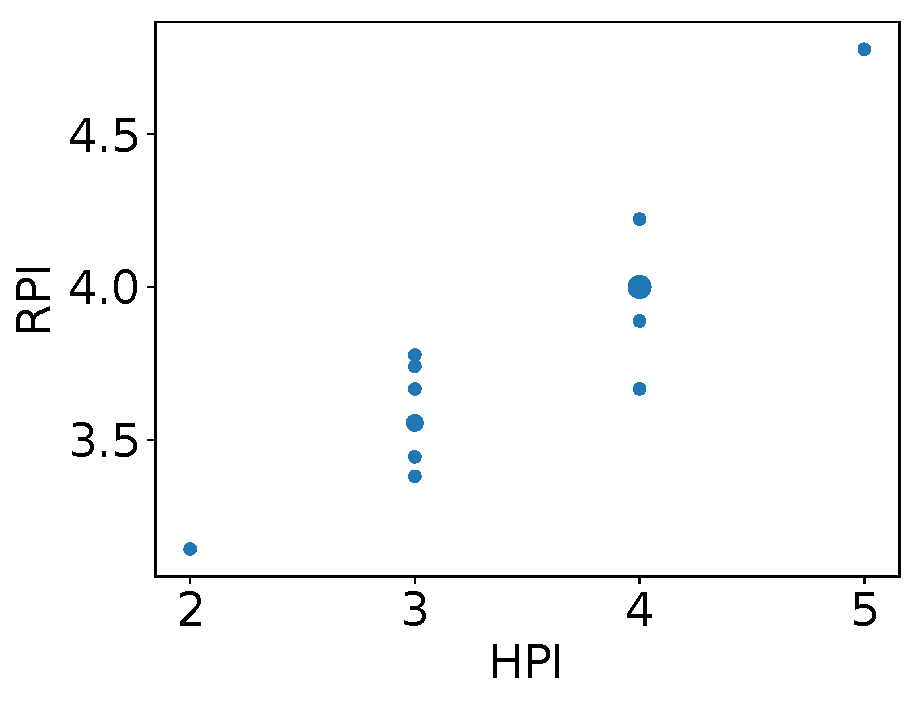
\includegraphics[width=0.24\textwidth]{figs/3-hk-auso-scatter}%
}%
}
\mbox{
\subfigure[4-AUSO]{%
\label{fig:auso4}%
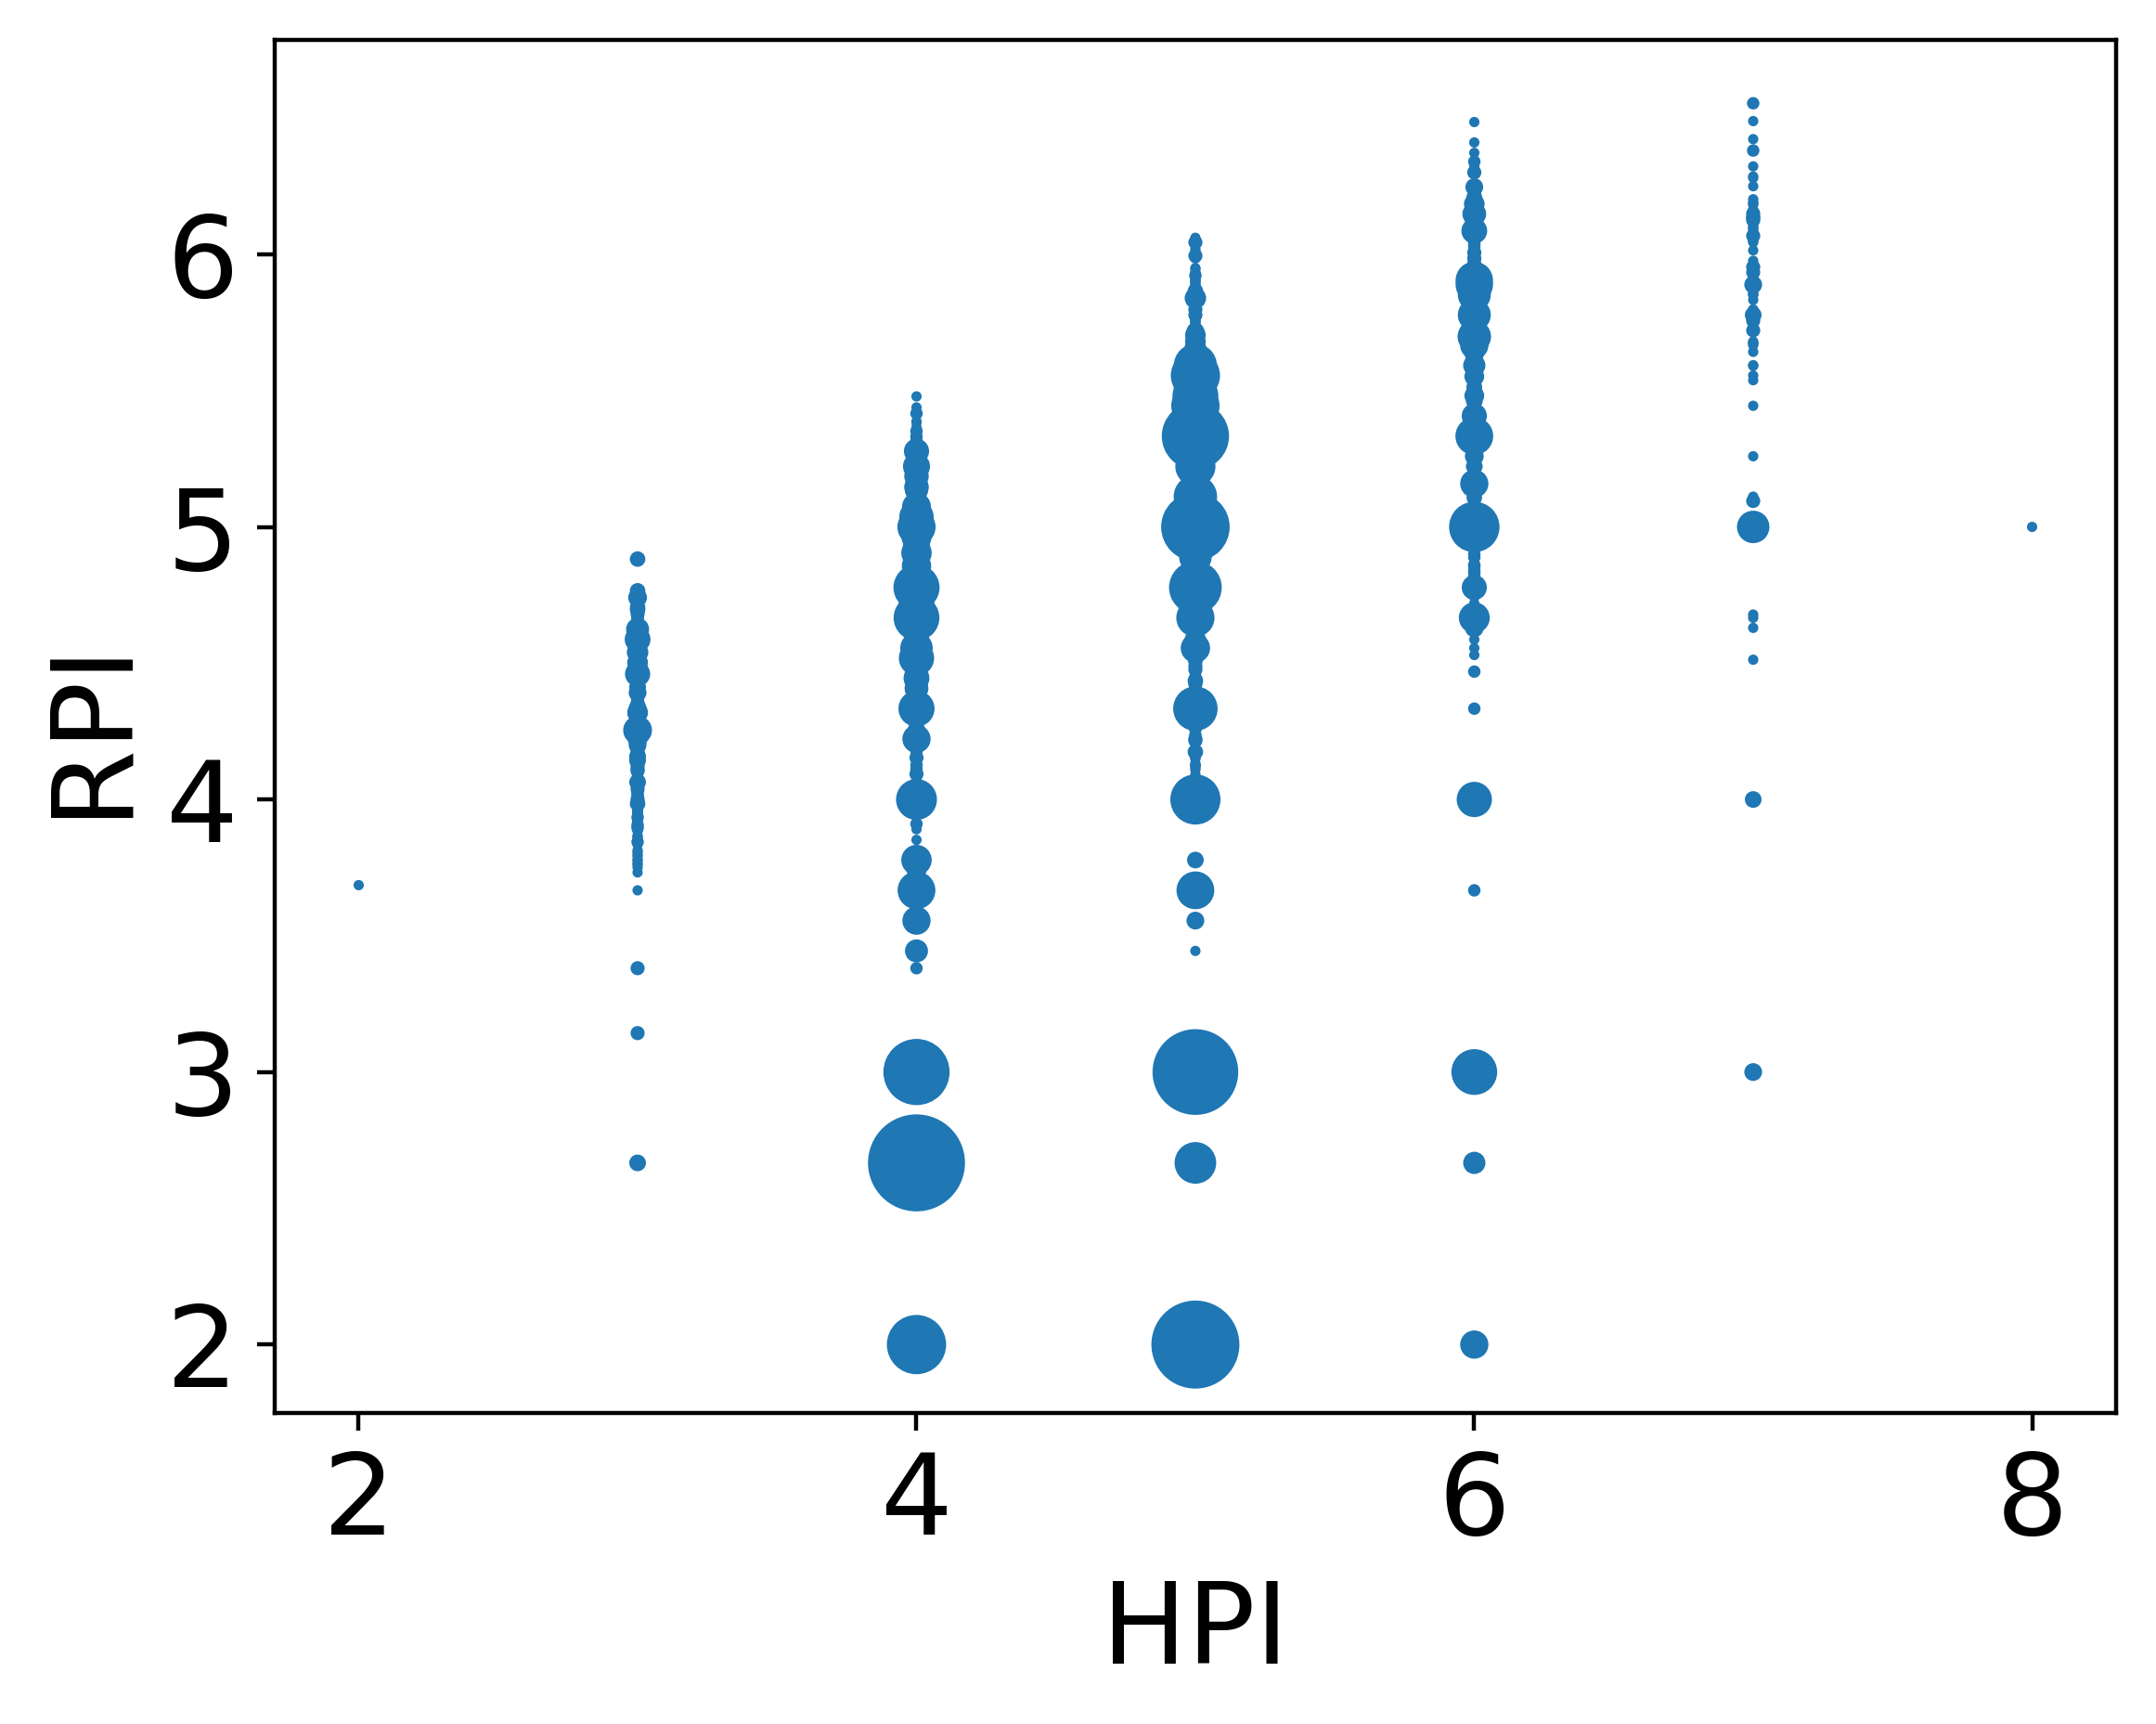
\includegraphics[width=0.24\textwidth]{figs/4-auso-scatter}%
}%
\subfigure[4-AUSO (Holt-Klee)]{%
\label{fig:hkauso4}%
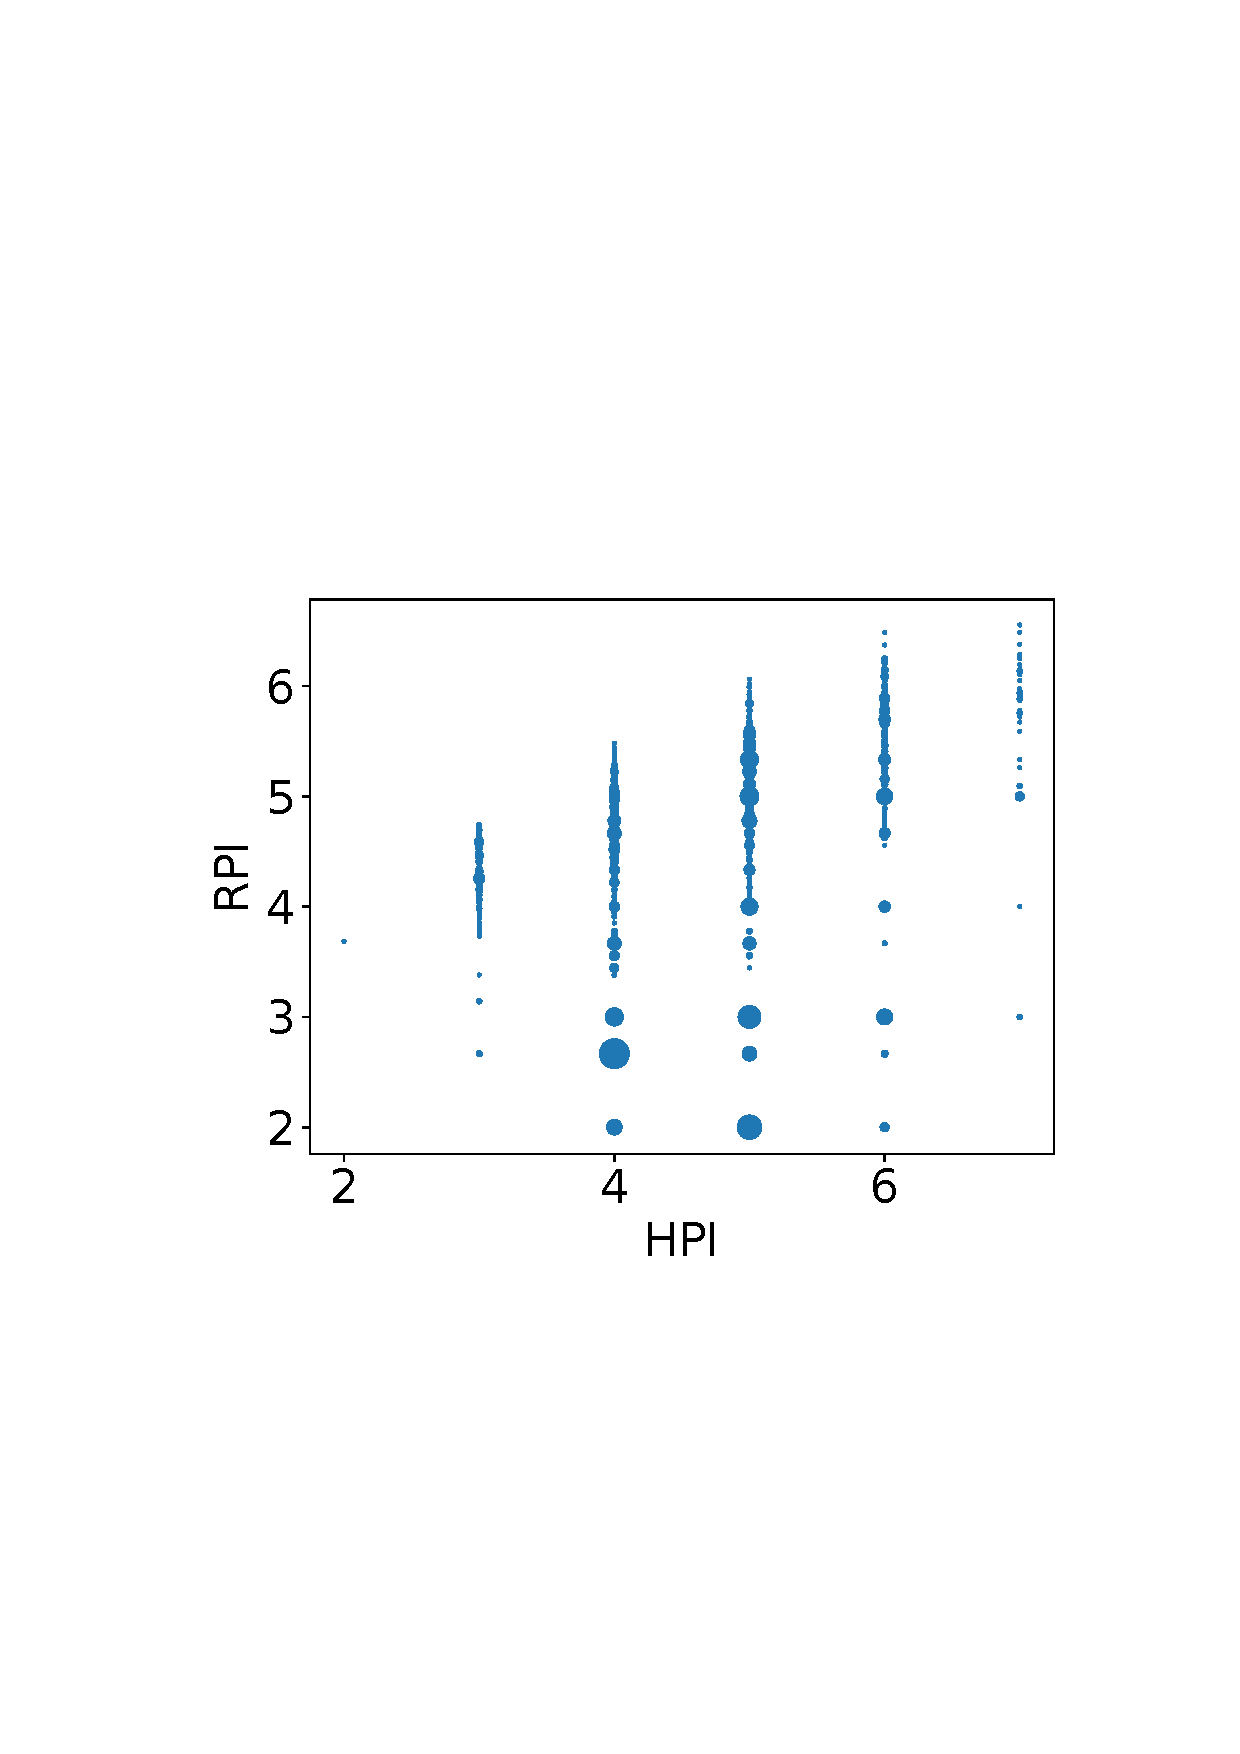
\includegraphics[width=0.24\textwidth]{figs/4-hk-auso-scatter}%
}%
}
\caption{Number of iterations taken by HPI and RPI on instances of different families of AUSOs. The area of each circle is proportional to the number of AUSOs whose HPI- and RPI- iterations are the centre's x and y coordinates, respectively. % For each method the curve is obtained by computing the number of iterations for each instance of the family, and plotting these numbers in non-decreasing order. Thus, for a given point on the x axis, the HPI and RPI iterations plotted might not be for the same instance.
}
\label{fig:3-4-auso-bounds}
\end{figure}


